\documentclass{article}
\usepackage{ctex}
\usepackage{amsmath}
\usepackage{graphicx}
\usepackage{wrapfig}
\usepackage{caption}
\usepackage[top=0.8in, bottom=0.8in,left=0.8in, right=0.8in]{geometry}
\usepackage{float} 
\usepackage{subfigure}
\usepackage{subcaption}
\usepackage{bm}
\xeCJKsetup{CJKmath=true} 

\begin{document}
\section*{悬链线(40分)(命题人:SCK)}
\[\]
(1)
\par
\begin{wrapfigure}{r}{4cm}
	\vspace{-15pt}    % 对应高度1
	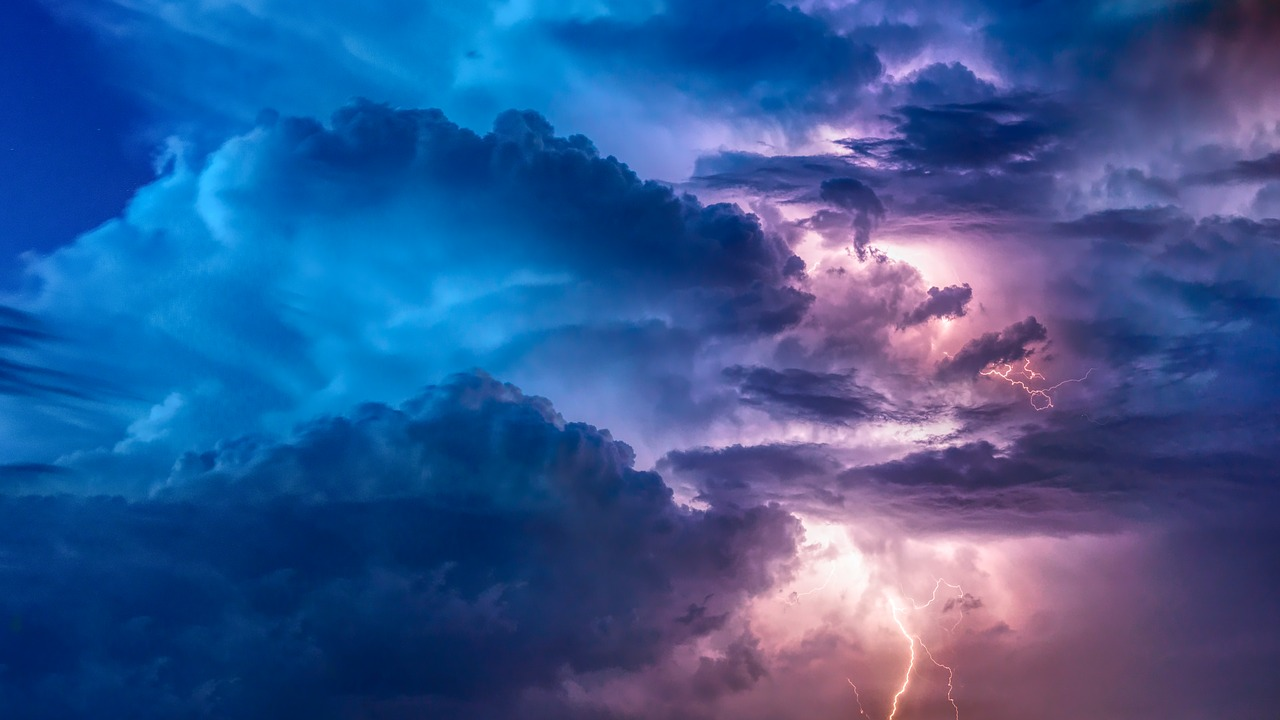
\includegraphics[width=4cm]{img/2.jpeg}\\
	\vspace{-15pt}    % 对应高度2
	\caption{}
	\vspace{-15pt}    % 对应高度3
\end{wrapfigure}
取微元受力分析
\[
\begin{cases}
    T\left( \theta +\mathrm{d}\theta \right) \sin \left( \theta +\mathrm{d}\theta \right) = \lambda g\mathrm{d}l+T(\theta)\sin \theta \\
    T\left( \theta +\mathrm{d}\theta \right) \cos \left( \theta +\mathrm{d}\theta \right) =T(\theta)\cos \theta 
\end{cases}
\tag{1}
\]
可得
\[
\begin{cases}
\mathrm{d}(T\sin(\theta))=\lambda g \sqrt{1+\left(\dfrac{\mathrm{d}y}{\mathrm{d}x}\right)^2}\mathrm{d}x\\
\mathrm{d}(T\cos(\theta))=0
\end{cases}
\tag{2}
\]
对(2)积分得:
\[
T\cos(\theta)=T_0
\tag{3}
\]
\[
T\sin(\theta)=T_0\dfrac{\mathrm{d}y}{\mathrm{d}x} 
\tag{4}
\]
联立(2)(4)
\[
T_{0}\dfrac{\mathrm{d}^{2}y}{\mathrm{d}x^{2}}=\lambda g\sqrt{1+\left(\dfrac{\mathrm{d}y}{\mathrm{d}x}\right)^2}
\tag{5}
\]
令$\dfrac{\mathrm{d}y}{\mathrm{d}x}=u$,得
\[
T_{0}\dfrac{\mathrm{d}u}{\mathrm{d}x}=\lambda g\sqrt{1+u^{2}}
\tag{6}
\]
\[
T_{0}\dfrac{\mathrm{d}u}{\mathrm{d}y}u=\lambda g\sqrt{1+u^{2}}
\tag{7}
\]
\[
T_{0}\dfrac{u\mathrm{d}u}{\sqrt{1+u^{2}}}=\lambda g\mathrm{d}y
\tag{8}
\]
注意到:$\mathrm{d}\left( \sqrt{1+u^{2}}\right) =\dfrac{u\mathrm{du}}{\sqrt{1+u^{2}}}$
\[
    T_0\mathrm{d}\left( \sqrt{1+u^{2}}\right) = +\lambda g\mathrm{d}y
\]
\[
    T_{0}\sqrt{1+u^{2}}-T_{0}=\lambda g\mathrm{d}y
\]
\[
    \sqrt{\left( \dfrac{T_{0}+\lambda gy}{T_{0}}\right) ^{2}-1}=\dfrac{\mathrm{d}y}{\mathrm{d}x}
\]
为了解上面的微分方程,注意到:
\[
\cosh^2 x-\sinh^2 x=1
\tag{9}
\]
令
\[
\dfrac{T_{0}+\lambda gy}{T_{0}}=\cosh \xi 
\tag{10}
\]
则上述方程化为
\[
\sinh \xi=\dfrac{\mathrm{d}y}{\mathrm{d}x}
\tag{11}
\]
对(10)求导
\[
\dfrac{\lambda g}{T_{0}}=\sinh \xi\dfrac{\mathrm{d}\xi}{\mathrm{d}y}
\tag{12}
\]
带入(11)
\[
\dfrac{\lambda g}{T_{0}}\dfrac{\mathrm{d}y}{\mathrm{d}\xi}=\dfrac{\mathrm{d}y}{\mathrm{d}x}
\tag{13}
\]
得到
\[
\xi=\dfrac{\lambda g}{T_{0}} x
\tag{14}
\]
可得
\[
y=\dfrac{T_0\left(\cosh\left(\dfrac{\lambda g}{T_{0}} x\right)-1\right)}{\lambda g}
\tag{15}
\]
(2)
\par
\begin{wrapfigure}{r}{4cm}
	\vspace{-15pt}    % 对应高度1
	
\includegraphics[width=4cm]{img/3.jpeg}\\
	\vspace{-15pt}    % 对应高度2
	\caption{}
	\vspace{-15pt}    % 对应高度3
\end{wrapfigure}
取微元受力分析,可得起沿着径向,有
\[
2T_0\frac{1}{2}\mathrm{d}=BI\mathrm{d}l
\tag{16}
\]
可得
\[
R=\dfrac{T_0}{BI}
\tag{17}
\]
可得方程
\[
x^2+\left(y-\dfrac{T_0}{BI}\right)^2=\left(\dfrac{T_0}{BI}\right)^2
\tag{18}
\]
(3)
\par
\begin{wrapfigure}{r}{4cm}
	\vspace{-15pt}    % 对应高度1
	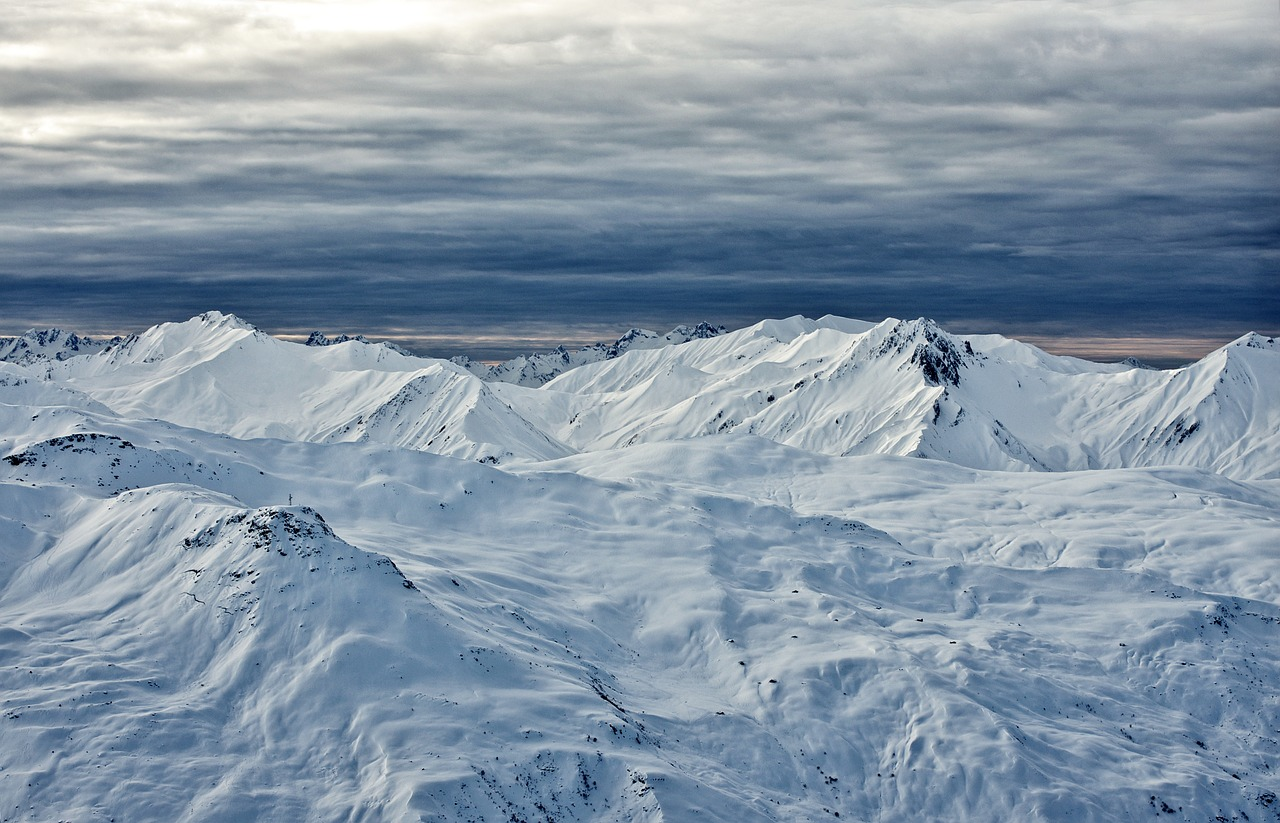
\includegraphics[width=4cm]{img/4.jpeg}\\
	\vspace{-15pt}    % 对应高度2
	\caption{}
	\vspace{-15pt}    % 对应高度3
\end{wrapfigure}
取微元受力分析
\[
\begin{cases}
    T\left( \theta +\mathrm{d}\theta \right) \sin \left( \theta +\mathrm{d}\theta \right) =BI\mathrm{d}l\cos \theta +\lambda g\mathrm{d}l+T(\theta)\sin \theta \\
    T\left( \theta +\mathrm{d}\theta \right) \cos \left( \theta +\mathrm{d}\theta \right) +BI\mathrm{d}l\sin \theta =T(\theta)\cos \theta 
\end{cases}
\tag{19}
\]
可得
\[
\begin{cases}
\mathrm{d}(T\sin(\theta))=BI\mathrm{d}x+\lambda g \sqrt{1+\left(\dfrac{\mathrm{d}y}{\mathrm{d}x}\right)^2}\mathrm{d}x\\
\mathrm{d}(T\cos(\theta))-BI\mathrm{d}y
\end{cases}
\tag{20}
\]
对(20)积分得:
\[
T\cos(\theta)=T_0-BIy
\tag{21}
\]
\[
T\sin(\theta)=(T_0-BIy)\dfrac{\mathrm{d}y}{\mathrm{d}x} 
\tag{22}
\]
联立(20)(22)
\[
T_{0}\dfrac{\mathrm{d}^{2}y}{\mathrm{d}x^{2}}-BI\left( \dfrac{\mathrm{d}y}{\mathrm{d}x}\right) ^{2}-BIy\dfrac{\mathrm{d}^{2}y}{\mathrm{d}x^{2}}=BI+\lambda g\sqrt{1+\left(\dfrac{\mathrm{d}y}{\mathrm{d}x}\right)^2}
\tag{23}
\]
令$\dfrac{\mathrm{d}y}{\mathrm{d}x}=u$,得
\[
T_{0}\dfrac{\mathrm{d}u}{\mathrm{d}x}-BIu^{2}-BIy\dfrac{\mathrm{d}u}{\mathrm{d}x}=BI+\lambda g\sqrt{1+u^{2}}
\tag{24}
\]
\[
T_{0}\dfrac{\mathrm{d}u}{\mathrm{d}y}u=BI\left(1+u^{2}\right)+BIyu\dfrac{\mathrm{d}u}{\mathrm{d}x}+\lambda g\sqrt{1+u^{2}}
\tag{25}
\]
\[
T_{0}\dfrac{u\mathrm{d}u}{\sqrt{1+u^{2}}}=BI\sqrt{1+u^{2}}\mathrm{d}y+BIy\dfrac{u\mathrm{d}u}{\sqrt{1+u^{2}}}+\lambda g\mathrm{d}y
\tag{26}
\]
注意到:$\mathrm{d}\left( \sqrt{1+u^{2}}\right) =\dfrac{u\mathrm{du}}{\sqrt{1+u^{2}}}$
\[
    T_0\mathrm{d}\left( \sqrt{1+u^{2}}\right) =BI\mathrm{d}\left( y\sqrt{1+u^{2}}\right) +\lambda g\mathrm{d}y
\tag{27}
\]
\[
    T_{0}\sqrt{1+u^{2}}-T_{0}=BI\mathrm{d}\left( y\sqrt{1+n^{2}}\right) +\lambda g\mathrm{d}y
    \tag{28}
\]
\[
    \sqrt{\left( \dfrac{T_{0}+\lambda gy}{T_{0}-BIy}\right) ^{2}-1}=\dfrac{\mathrm{d}y}{\mathrm{d}x}
    \tag{29}
\]
\textbf{评分标准:}\par
共$40$ 分\par
(1)共$15$分 $(1),(2),(3),(4),(5),(6),(7),(8),(9),(10),(11),(12),(13),(14),(15)$各$1$分\par
(2)共$5$分 $(16)$各$1$分,$(17),(18)$各$2$分\par
(3)共$20$分 $(19),(20),(21),(22),(23),(24),(25),(26),(27),(28),(29),(30),(31),(32),(33)$各$2$分\par
\end{document}